% Kozierok, ch. 16
\chapter{IPv4 addressing concepts and issues}
\label{chap:kozierok-ch16}

The primary job of the Internet Protocol is delivering messages between devices, and like any good delivery service, it can't do its job
too well if it doesn't know where the recipients are located.
Obviously then, one of the most important functions of IP is \emph{addressing}.
IP addressing is used not only to uniquely identify IP addresses, but also to facilitate the routing of IP datagrams over internetworks.
IP addresses are used and referred to extensively in TCP/IP networking.

Even though the original IP addressing scheme was relatively simple, it has become complex over time as changes have been made to it to allow it
to deal with various addressing requirements.
The more advanced styles of IP addressing, such as subnetting and classless addressing, are the ones used most in modern networks.
However, they can be a bit confusing to understand.
To help make sense of them, we must start at the beginning with a discussion of the fundamentals of IP addressing.

In this chapter, I begin a larger exploration of IP addressing
by explaining the key concepts and issues behind it. I begin with an
overview of IP addressing and a discussion of what it is all about. I
describe the size of IP addresses, the concept of its address space, and
the notation usually used for IP addresses. I provide basic information
on the structure of an IP address and how it is divided into a network
identifier and host identifier. I then describe the different types of
IP addresses and the additional information, such as a subnet mask and
default gateway, that often accompanies an IP address on larger
networks. I provide a brief description of how multiple addresses are
sometimes assigned to single devices and why. I conclude with a
description of the process by which public IP addresses are registered
and managed, and the organizations that do this work for the global
Internet.

\begin{backgroundinfo}
If you are not familiar with at least the basics of how binary numbers work, and also with how to
convert between binary and decimal numbers, I recommend reading \vref{chap:binary-numbers}, which provides some background
on data representation and the mathematics of computing, before you proceed here.
\end{backgroundinfo}




\section{IP addressing overview and fundamentals}


IP addressing is important because it facilitates the primary function of the Internet Protocol: the delivery of datagrams across an internetwork.
When you examine this in more detail, it becomes apparent that the IP address actually has two different functions, as follows:
\begin{description}
   \item[Network interface identification]
      Like a street address, the IP address provides unique identification of the interface between a device and the network.
      This is required to ensure that the datagram is delivered to the correct recipients.
   \item[Routing]
      When the source and destination of an IP datagram are not on the same network, the datagram must be delivered indirectly using intermediate systems.
      This is a process called \emph{routing}.
      The IP address is an essential part of the system used to route datagrams.
\end{description}

You may have noticed a couple of things about this short list.
One is that I said the IP address identifies the {\emph{network interface}},
not that it identifies the \emph{device} itself. This distinction is
important because it underscores the concept that IP is oriented around
connections to a large, virtual network at layer~3, which can span multiple physical networks.
Some devices, such as routers, will have more than one network connection, necessary to take datagrams from one network and route them onto another.
This means they will also have more than one IP address -- one per connection.

You might also find it curious that I said that the IP address facilitates routing.
How can it do that?
The answer is that the addressing system is designed with a structure that can be interpreted to allow routers to determine what to do with a datagram based on the values in the address.
Numbers related to the IP address, such as the subnet mask when subnetting is used, support this function.

Let's look at some of the more important issues and characteristics associated with IP addresses in general terms.



\subsection{Number of IP addresses per device}

Any device that has data sent to it at the network layer will have at
least one IP address: one per network interface. This means that normal
hosts such as computers and network-capable printers usually get one IP
address, while routers get more than one IP address. Some special hosts
may have more than one IP address if they are multihomed -- connected to more than one network.

Lower-level network interconnection devices -- such as repeaters,
bridges, and switches -- don't require an IP address because they pass
traffic based on layer~2 (data link layer) addresses. Network segments
connected by bridges and switches form a single \emph{broadcast domain}, and any devices on them can send data to each other directly without routing.
To IP, these devices are essentially invisible; they are no
more significant than the wires that connect devices together (with a
couple of exceptions). Such devices may, however, optionally have an IP
address for management purposes. In this regard, they are acting like a
regular host on the network.

\Cref{fig:ip-interfaces} shows the IP interfaces of a few common LAN devices as small circles.
Each regular host has one interface, while the router that serves this LAN has three, since it connects to three different networks.
Note that the LAN switch has no IP interfaces; it connects the hosts and router at layer~2.
(Also see Figure~16-5, which shows the IP interfaces of devices in a more complex configuration.)


\begin{figure}
   \centering
   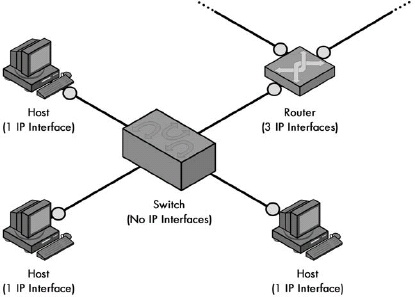
\includegraphics[width=.6\textwidth]{images/ip-interfaces.jpg}
   \caption{IP interfaces for common network devices -- Regular hosts have one interface; routers usually have more than one; and switches have none (because they operate at layer~2).}
   \label{fig:ip-interfaces}
\end{figure}



\subsection{Address uniqueness and network specificity}

Each IP address on a single internetwork must be unique.
(This seems rather obvious, although there are exceptions in IPv6,\footnote{As well as in IPv4.} in the form of special anycast addresses, as discussed in \protect\hyperlink{ch25.html}{Chapter~25}.)

Since IP addresses represent network interfaces and are used for routing, the IP address is
specific to the network to which it is connected.
If the device moves to a new network, the IP address will usually have to change as well.
For the full reason why, see the discussion of basic IP address structure later in this chapter.
This issue was a primary motivation for the creation of Mobile IP.% (covered in \protect\hyperlink{ch30.html}{Chapter~30}).



\subsection{Contrasting IP addresses and data link layer addresses}

IP addresses are used for network-layer data delivery across an internetwork. This
makes IP addresses quite different from the data link layer address of a
device, such as its Ethernet MAC address. (In TCP/IP parlance, these are
sometimes called \emph{physical addresses} or \emph{hardware addresses}.)

At the network layer, a single datagram may be sent from device~A to device~B.
However, the actual delivery of the datagram may require that it passes through a dozen or more physical devices if device~A and device~B are not on the same network.

It is also necessary to provide a function that maps between IP and data link layer addresses.
In TCP/IP, this is the job of the Address Resolution Protocol (ARP; see \protect\hyperlink{ch13.html}{Chapter~13}).

In a physical network such as an Ethernet, the MAC address is all the
information needed to send data between devices. In contrast, an IP
address represents only the final delivery point of the datagram. The
route taken depends on the characteristics of the network paths between
the source and destination devices. It is even possible that there may
not be a route between any two devices, which means two devices cannot
exchange data, even if they know each other's addresses!



\subsection{Private and public IP network addresses}

There are two distinct ways that a network can be set up with IP addresses.
On a {\emph{private network}}, a single organization controls the assignment of the addresses for all devices; they have pretty much absolute control to do what they wish in selecting numbers, as long as each address is unique.

In contrast, on a {\emph{public network}}, a mechanism is required to ensure that organizations don't use overlapping addresses and that they enable efficient routing of data between organizations.
The best-known example of this is the Internet, where public IP registration and management facilities have been created to address this issue.
There are also advanced techniques now, such as IP network address translation (NAT), which allow a network using private addresses to be interfaced to a public TCP/IP network.



\subsection{IP address configuration and addressing types}

IP addresses can be set up as either a static or dynamic configuration.
In a {\emph{static configuration}} setup, each device is manually configured with an IP address that doesn't change.
This is fine for small networks but quickly becomes an administrative nightmare in larger networks, when changes are required.
The alternative, {\emph{dynamic configuration}}, allows IP addresses to be assigned to devices and changed under software control.
The two host configuration protocols, BOOTP and DHCP, were created to fill this latter function.
% (see \protect\hyperlink{pt14.html}{Part~III-3}).
We will not cover BOOTP as it is too old but will cover DHCP in \vref{chap:dhcp}.

Additionally, provision is included in the IP addressing scheme for all three basic types of addressing: unicast, multicast, and broadcast.
And, contrary to popular belief, IPv4 \emph{also} supports anycast addressing.

\begin{keyconcept}
IP addresses serve the dual function of device identification and routing.
Each network interface requires one IP address, which is network specific.
IP addresses can be either statically or dynamically allocated, and come in unicast, multicast, and broadcast forms, and with support for anycast routing.
\end{keyconcept}


\section{IP address size, address space, and notation}

Now that you have looked at the general issues and characteristics
associated with IP addresses, it's time to get past the introductions
and dig into the ``meat'' of the IP address discussion.
Let's start by looking at the physical construction and size of the IP address and how it is referred to and used.


\subsection{IP address size and binary notation}

At its simplest, the IP address is just a 32-bit binary number: a set of 32 ones or zeros. At their lowest levels, computers always work in binary,
and this also applies to networking hardware and software. While
different meanings are ascribed to different bits in the address, the
address itself is just a 32-digit binary number.

People don't work too well with binary numbers, because they are long
and complicated, and the use of only two digits makes them hard to
differentiate. (Quick, which of these is larger:
11100011010100101001100110110001 or 11100011010100101001101110110001?)
For this reason, when you use IP addresses, you don't work with them in
binary except when absolutely necessary.

The first thing that people would naturally do with a long string of bits is to split it into four eight-bit octets (or bytes, even though
the two aren't technically the same; see \vref{chap:binary-numbers}), to make it more manageable.
So 1110\-0011\-0101\-0010\-1001\-1011\-1011\-0001 would become 11100011 - 01010010 -
10011101 - 10110001. Then you could convert each of those octets into a
more manageable two-digit hexadecimal number to yield the following: E3
- 52 - 9D - B1. This is, in fact, the notation used for IEEE 802 MAC
addresses, except that they are 48 bits long, so they have six two-digit
hex numbers, and they are usually separated by colons, not dashes, as I
used here.

(Incidentally, the second binary number is the larger one.)



\subsection{IP address dotted decimal notation}

Most people still find hexadecimal a bit difficult to work with.
So, IP addresses are normally expressed with each octet of eight bits converted to a
decimal number and the octets separated by a period (a \emph{dot}).
Thus, the previous example would become 227.82.157.177, as shown in \cref{fig:ip-address-notation}.
This is usually called {\emph{dotted decimal notation}} for rather
obvious reasons. Each of the octets in an IP address can take on the
values from 0 to 255, so the lowest value is theoretically 0.0.0.0 and
the highest is 255.255.255.255.

\begin{keyconcept}
IP addresses are 32-bit binary numbers, which can be expressed in binary, hexadecimal, or decimal form.
Most commonly, they are expressed by dividing the 32 bits into four octets and converting each to decimal, then separating these numbers with dots to create dotted decimal notation.
\end{keyconcept}


\begin{figure}
   \centering
   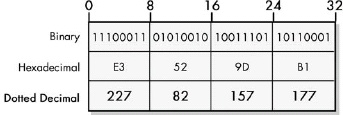
\includegraphics[width=.7\textwidth]{images/ip-address-notation.jpg}
   \caption
      [IP address binary, hexadecimal, and dotted decimal representations]
      {IP address binary, hexadecimal, and dotted decimal representations -- The binary, hexadecimal, and decimal representations of an IP address are all equivalent.}
   \label{fig:ip-address-notation}
\end{figure}

Dotted decimal notation provides a convenient way to work with IP addresses when communicating among people.
Never forget that to the computers, the IP address is always a 32-bit binary
number; you'll understand the importance of this when you look at how
the IP address is logically divided into components in the next topic,
and when you examine techniques that manipulate IP addresses, such as
subnetting.



\subsection{IP address space}

Since the IP address is 32 bits wide, this provides a theoretical {\emph{address
space}} of $2^{32}$, or 4,294,967,296 addresses.
This seems like quite a lot of addresses, and in some ways, it is.
However, as you will see, due to how IP addresses are structured and allocated, not every one of those addresses can actually be used.

One of the unfortunate legacies of the fact that IP was originally
created on a rather small internetwork is that decisions were made that
wasted much of the address space. For example, all IP addresses starting
with 127 in the first octet are reserved for the loopback function. Just
this one decision makes 1/256th of the total number, or 16,277,216
addresses, no longer available. There are also other ways that the IP
address space was not conserved. This caused difficulty as the Internet
grew in size. (You'll see more about this in \vref{chap:kozierok-ch17}, which covers classful addressing.)


\begin{keyconcept}
Since IP addresses are 32 bits long, the total address space of IPv4 is $2^{32}$ or 4,294,967,296 addresses.
However, not all of these addresses can be used, for a variety of reasons.
\end{keyconcept}

This IP address space dictates the limit on the number of addressable
interfaces in \emph{each} IP internetwork. So, if you have a private
network, you can, in theory, have four-billion-plus addresses. However,
in a public network such as the Internet, all devices must share the
available address space. Techniques such as \emph{classless inter-domain routing} (CIDR), or \emph{supernetting}, and NAT were designed in part to
utilize the existing Internet IP address space more efficiently.
IPv6 expands the IP address size from 32 bits all the way up to 128, which increases the address space to a ridiculously large number and makes the entire matter of address space size moot.



\section{IP basic address structure and main components}

As I mentioned in the IP addressing overview, one of the ways that IP addresses are used is to facilitate the routing of datagrams in an IP internetwork.
This is made possible because of the way that IP addresses are structured and how that structure is interpreted by network routers.



\subsection{Network ID and host ID}

As you just saw, each IPv4 address is 32 bits long.
When you refer to the IP address, you use a dotted decimal notation, while the computer converts
this into binary. However, even though these sets of 32 bits are
considered a single entity, they have an internal structure containing
two components:
\begin{description}
   \item[Network identifier (network ID)]
      A certain number of bits, starting from the leftmost bit, is used to identify the network where the host or other network interface is located. This is also sometimes called the \emph{network prefix} or even just the \emph{prefix}.
   \item[Host identifier (host ID)]
      The remainder of the bits is used to identify the host on the network.
\end{description}

\begin{note}
By convention, IP devices are often called hosts for simplicity, as I do throughout this book.
Even though each host usually has a single IP address, you should remember that IP addresses are strictly associated with network layer network interfaces,
not physical devices, and a device may therefore have more than one IP address (especially a router or multihomed host).
\end{note}

As you can see in \cref{fig:ip-address-division},
this really is a fairly simple concept. The fundamental division of the
bits of an IP address is into a network ID and host ID. In this
illustration, the network ID is 8 bits long, and the host ID is 24 bits
in length. This is similar to the structure used for phone numbers in
North America. The telephone number (401) 555-7777 is a ten-digit number
that's usually referred to as a single phone number. However, it has a
structure. In particular, it has an area code (401) and a local number
(555-7777).

The fact that the network ID is contained in the IP address is what
partially facilitates the routing of IP datagrams when the address is
known. Routers look at the network portion of the IP address to first
determine if the destination IP address is on the same network as the
host IP address. Then routing decisions are made based on information
the routers keep about where various networks are located. Again, this
is conceptually similar to how the area code is used by the equivalent
of routers in the phone network to switch telephone calls. The host
portion of the address is used by devices on the local portion of the
network.

\begin{figure}
   \centering
   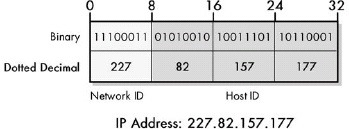
\includegraphics[width=.6\textwidth]{images/ip-address-division.jpg}
   \caption
      [Basic IP address division: network ID and host ID]
      {Basic IP address division: network ID and host ID -- This diagram shows one of the many ways to divide an IP address into a network ID and host ID.}
   \label{fig:ip-address-division}
\end{figure}



\subsection{Location of the division between network ID and host ID}

One difference between IP addresses and phone numbers is that the
dividing point between the bits used to identify the network and those
that identify the host isn't fixed. It depends on the nature of the
address, the type of addressing being used, and other factors.

Take the previous example of 227.82.157.177 (see \vref{fig:ip-address-notation}).
It is possible to divide this into a network ID of 227.82 and a host ID of 157.177.
Alternatively, the network ID might be 227 and the host ID might be 82.157.177 within that network.

To express the network and host IDs as 32-bit addresses, you add zeros
to replace the missing pieces. With a network ID of 227 and a host ID of
82.157.177, the address of the network becomes 227.0.0.0 and the address
of the host 0.82.157.177.
(In practice, network addresses of this sort are routinely seen with the added zeros; host IDs are not seen as often in 32-bit form this way.)

Lest you think from these examples that the division
must always be between whole octets of the address, you should know that
it's also possible to divide it in the middle of an octet. For example,
you could split the IP address 227.82.157.177 so that there were 20 bits
for the network ID and 12 bits for the host ID. The process is the same,
but determining the dotted decimal ID values is more tricky because
here, the 157 is split into two binary numbers. The results are
227.82.144.0 for the network ID and 0.0.0.13.177 for the host ID, as
shown in \cref{fig:slash-20}.

Since IP addresses are normally expressed as four dotted-decimal
numbers, educational resources often show the division between the
network ID and host ID occurring on an octet boundary. However, it's
essential to remember that the dividing point often appears in the
middle of one of these eight-bit numbers.
In \cref{fig:slash-20}, the network ID is 20~bits long, and the host ID 12~bits long.
This results in the third number of the original IP address,~157, being split into~144 and~13.

The place where the line is drawn between the network ID and the host ID
must be known in order for devices such as routers to know how to
interpret the address. This information is conveyed either implicitly or
explicitly, depending on the type of IP addressing in use, as I discuss
next.


\begin{figure}
   \centering
   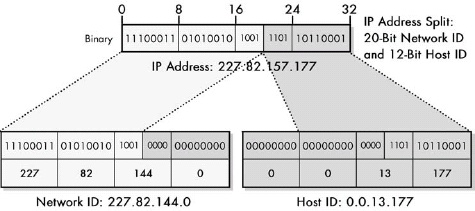
\includegraphics[width=.6\textwidth]{images/slash-20.jpg}
   \caption
      [Mid-octet IP address division]
      {Mid-octet IP address division -- IP addresses need not be divided between network ID and host ID on octet boundaries.
      The division here is into a 20-bit network ID and a 12-bit host ID.}
   \label{fig:slash-20}
\end{figure}


\begin{keyconcept}
The basic structure of an IP address consists of two components: the network ID and host ID.
The dividing point of the 32-bit address is not fixed, but depends on a number of factors and can occur in a variety of places, including in the middle of a dotted-decimal octet.
\end{keyconcept}

Since the IP address can be split into network ID and host ID
components, it is also possible to use either one or the other by
itself, depending on context. These addresses are assigned special
meanings. For example, if the network ID is used with all ones as the
host ID, this indicates a broadcast to the entire network. Similarly, if
the host ID is used by itself with all zeros for the network ID, this
implies an IP address sent to the host of that ID on the local network,
whatever that might be.
This is explained in much more detail in \vref{chap:kozierok-ch17}.

It is the inclusion of the network ID in the IP address of each host on
the network that causes the IP addresses to be network-specific. If you
move a device from one network to a different one, the network ID must
change to that of the new network. Therefore, the IP address must change
as well. This is an unfortunate drawback that shows up most commonly
when dealing with mobile devices; see
\protect\hyperlink{ch30.html}{Chapter~30}.


\section{IP addressing categories and IP address adjuncts}

We just explored how the 32 bits in an IP address are fundamentally divided into
the network ID and host ID. The network ID is used for routing purposes,
and the host ID uniquely identifies each network interface on the
network. In order for devices to know how to use IP addresses on the
network, they must be able to tell which bits are used for each ID.
However, the dividing line is not predefined. It depends on the type of
addressing used in the network.

Understanding how these IDs are determined leads us into a larger
discussion of the three main categories of IP addressing schemes:
classful, subnetted, and classless. Each of these uses a slightly
different system of indicating where in the IP address the host ID is
found.



\subsection{Conventional (classful) addressing}

The original IP addressing scheme is set up so that the dividing line
occurs only in one of a few locations: on octet boundaries. Three main
classes of addresses -- A, B, and C -- are differentiated based on how
many octets are used for the network ID and how many for the host ID.
For example, class C addresses devote 24 bits to the network ID and 8
bits to the host ID. This type of addressing is now often referred to by
the made-up word \emph{classful} to differentiate it from the newer
classless scheme.

This most basic addressing type uses the simplest method to divide the
network and host IDs: The class, and therefore the dividing point, are
encoded into the first few bits of each address. Routers can tell from
these bits which octets belong to which identifier.




\subsection{Subnetted classful addressing}

In the subnet addressing system, the two-tier network and host division
of the IP address is made into a three-tier system by taking some number
of bits from a class A, B, or C host ID and using them for a
{\emph{subnet identifier (subnet ID)}}. The network ID is unchanged. The
subnet ID is used for routing within the different subnetworks that
constitute a complete network, thereby providing extra flexibility for
administrators. For example, consider a class C address that normally
uses the first 24 bits for the network ID and remaining 8 bits for the
host ID. The host ID can be split into, say, 3 bits for a subnet ID and
5 bits for the host ID.

This system is based on the original classful scheme, so the dividing
line between the network ID and full host ID is based on the first few
bits of the address as before. The dividing line between the subnet ID
and the ``subhost'' ID is indicated by a 32-bit number called a
{\emph{subnet mask}}. In the previous example, the subnet mask would be
27 ones followed by 5 zeros -- the zeros indicate what part of the
address is the host. In dotted decimal notation, this would be
255.255.255.224.




\subsection{Classless addressing}

In the classless system, the classes of the original IP addressing
scheme are tossed out the window. The division between the network ID
and host ID can occur at an arbitrary point, not just on octet
boundaries, as in the classful scheme.

The dividing point is indicated by putting the number of bits used for
the network ID, called the {\emph{prefix length}}, after the address.
(Recall that the network ID bits are also sometimes called the
{\emph{network prefix}}, so the network ID size is the prefix length.)
For example, if 227.82.157.177 is part of a network where the first 27
bits are used for the network ID, that network would be specified as
227.82.157.160/27. The /27 is conceptually the same as the
255.255.255.224 subnet mask, since it has 27 one bits followed by 5
zeros.


\begin{keyconcept}
An essential factor in determining how an IP address is interpreted is the addressing scheme in which it is used.
The three methods, arranged in increasing order of age, complexity, and flexibility, are classful addressing, subnetted classful addressing, and classless addressing.
\end{keyconcept}

This introduction to the concepts of classful, subnetted, and classless
addressing was designed to show you how they impact the way the IP
address is interpreted. I have greatly summarized important concepts
here. All three methods are explained in their own chapters in full
detail.




\subsection{Subnet mask and default gateway}

In the original classful scheme, the division between network ID and host ID is
implied.
However, if either subnetting or classless addressing is used, then the {\emph{subnet mask}} (or {\emph{slash number}}, which is equivalent) is required to fully qualify the address.
These numbers are considered adjuncts to the IP address and usually mentioned with the address itself, because without them, it is not possible to know where the network ID ends and the host ID begins.

One other number that is often specified along with the IP address for a device is the \emph{default gateway} identifier.
In simplest terms, this is the IP address of the
router that provides default routing functions for a particular device.
When a device on an IP network wants to send a datagram to a device it
can't see on its local IP network, it sends it to the default gateway,
which takes care of routing functions. Without this, each IP device
would also need to have knowledge of routing functions and routes, which
would be inefficient. See \protect\hyperlink{ch23.html}{Chapter~23},
which discusses IP routing concepts, and
\protect\hyperlink{ch37.html}{Chapter~37} through 41, which cover TCP/IP
routing protocols, for more information.


\section{Number of IP addresses and multihoming}
Each network interface on an IP internetwork has a separate IP address.
In a classic network, each regular computer, usually called a
\emph{host}, attaches to the network in exactly only one place, so it
will have only one IP address. This is what most of us are familiar with
when using an IP network (and is also why most people use the term
\emph{host} when they really mean {\emph{network interface}}).

If a device has more than one interface to the internetwork, it will
have more than one IP address. The most obvious case where this occurs
is with routers, which connect together different networks and thus must
have an IP address for the interface on each one. It is also possible
for hosts to have more than one IP address, however. Such a device is
sometimes said to be \emph{multihomed}.

There are two ways that a host can be multihomed:
\begin{description}
   \item[Two or more interfaces to the same network]
      Devices such as servers or high-powered workstations may be equipped with two physical interfaces to the same network for performance and reliability reasons.
      They will have two IP addresses on the same network with the same network ID.

   \item[Interfaces to two or more different networks]
      Devices may have multiple interfaces to different networks.
      The IP addresses will typically have different network IDs in them.
\end{description}


\Vref{fig:multihomed-devices} shows examples of both types of multihomed device.
Of course, these could be combined, with a host having two connections to one network and a third to another network.
There are also some other special cases, such as a host with a single network connection having multiple IP address aliases.

\begin{note}
When subnetting is used, the same distinction can be made between multihoming to the same subnet or a different subnet.
\end{note}

Now, let's consider the second case. If a host has interfaces to two or
more different networks, could it pass IP datagrams between them? Yes,
if it had the right software
running on it. And wouldn't that make the host a router, of sorts? In
fact, that is exactly the case. A multihomed host with interfaces to two
networks can use software to function as a router. This is sometimes
called \emph{software routing}.

Using a host as a router has certain advantages and disadvantages
compared to a hardware router. A server that is multihomed can perform
routing functions and also, well, act as a server. A dedicated hardware
router is designed for the job of routing and usually will be more
efficient than a software program running on a host.


\begin{keyconcept}
A host with more than one IP network interface is said to be multihomed.
A multihomed device can have multiple connections to the same network, to different networks, or both.
A host connected to two networks can be configured to function as a router.
\end{keyconcept}


Multihoming was once considered a fairly esoteric application, but has
become more common in recent years. This is also true of multihoming on
different networks for software routing use. In fact, you may be doing
this in your home without realizing it.

Suppose you have two PCs networked together and a single phone line to
connect to the Internet. One computer dials up to your Internet service
provider (ISP) and runs software such as Microsoft's Internet
Connection Sharing (ICS) to
let the other computer access the Internet. Millions of people do this
every day -- they have a multihomed system (the one connecting to the
Internet and the other PC) with ICS acting in the role of a software
router (though there are some technical differences between ICS and a
true router, of course).


\section{IP address management and assignment methods and authorities}
What would happen if you told someone that you lived at 34 Elm Street, and when he
turned onto your road, he found four different houses with the number 34
on them? He probably would find your place eventually but wouldn't be
too pleased. Neither would you or your mail carrier! And all of you
folks are much smarter than computers. Like street addresses, IP
addresses must be unique for them to be useful.


\begin{figure}
   \centering
   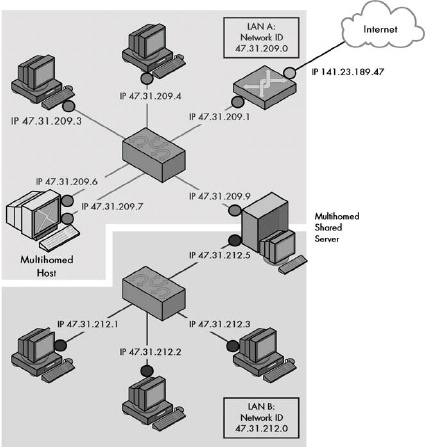
\includegraphics[width=\textwidth]{images/multihomed-devices.jpg}
   \caption
      [Multihomed devices on an IP internetwork]
      {Multihomed devices on an IP internetwork -- This internetwork consists of two LANs, A (above) and B (below).
      LAN A has a multihomed workstation, shown with two IP network interface ``circles.''
      The two LANs are connected together through a multihomed, shared server that has been configured to route traffic between them.
      Note that this server also handles all traffic passing between LAN B and the Internet (since the Internet connection is in LAN A only).
      }
   \label{fig:multihomed-devices}
\end{figure}


Since IP datagrams are sent only within the confines of the IP
internetwork, they must be unique within each internetwork. If you are a
company with your own private internetwork, this isn't really a big
problem. Whoever is in charge of maintaining the internetwork keeps a
list of what numbers have been used where and makes sure that no two devices are
given the same address. However, what happens in a public network with
many different organizations? Here, it is essential that the IP address
space be managed across the organizations to ensure that they use
different addresses. It's not feasible to have each organization
coordinate its activities with each other one. Therefore, some sort of
centralized {\emph{management authority}} is required.

At the same time that you need someone to ensure that there are no
conflicts in address assignment, you don't want users of the network to
have to go to this central authority every time they need to make a
change to their network. It makes more sense to have the authority
assign numbers in blocks or chunks to organizations based on the number
of devices they want to connect to the network. The organizations can
manage those blocks as they see fit, and the authority's job is made
easier because it deals in blocks instead of billions of individual
addresses and machines.

The Internet, as the big IP internetwork, requires this coordination
task to be performed for millions of organizations worldwide. The job of
managing IP address assignment on the Internet was originally carried
out by a single organization: the {\emph{Internet Assigned Number
Authority (IANA)}}. IANA was responsible for allocating IP addresses,
along with other important centralized coordination functions such as
managing universal parameters used for TCP/IP protocols. In the late
1990s, a new organization called the {\emph{Internet Corporation for
Assigned Names and Numbers (ICANN)}} was created.
ICANN now oversees the IP address assignment task of IANA, as well as managing other tasks such as Domain Name System (DNS) name registration (see \vref{chap:dns}).

IP addresses were originally allocated directly to organizations.
The original IP addressing scheme was based on classes, and so IANA would assign addresses in class A, B, and C blocks.
Today, addressing is classless, using CIDR's hierarchical addressing scheme.
IANA doesn't assign addresses directly, but rather delegates them to regional Internet registries (RIRs).
These are APNIC, ARIN, LACNIC, and RIPE NCC.
Each RIR can, in turn, delegate blocks of addresses to lower-level registries such as national Internet registries (NIRs) and local Internet registries (LIRs).

Eventually, blocks of addresses are obtained by ISPs for distribution to
end-user organizations. Some of the ISP's customers are end-user
organizations, but others are (smaller) ISPs themselves. They can, in
turn, use or delegate the addresses in their blocks. This can continue
for several stages in a hierarchical fashion. This arrangement helps
ensure that IP addresses are assigned and used in the most efficient
manner possible. See \vref{chap:kozierok-ch20}, which discusses CIDR, for more information on how this works.

IANA, ICANN, and the RIRs are responsible for more than just IP address allocation, though I have concentrated on IP addresses here for obvious reasons.
For more general information on IANA, ICANN, APNIC, ARIN, LACNIC, and RIPE NCC, try a can of alphabet soup
-- or \protect\hyperlink{ch03.html}{Chapter~3}, which provides an overview of the Internet registration authorities.

